\documentclass{article}\usepackage[]{graphicx}\usepackage[]{color}
%% maxwidth is the original width if it is less than linewidth
%% otherwise use linewidth (to make sure the graphics do not exceed the margin)
\makeatletter
\def\maxwidth{ %
  \ifdim\Gin@nat@width>\linewidth
    \linewidth
  \else
    \Gin@nat@width
  \fi
}
\makeatother

\definecolor{fgcolor}{rgb}{0.345, 0.345, 0.345}
\newcommand{\hlnum}[1]{\textcolor[rgb]{0.686,0.059,0.569}{#1}}%
\newcommand{\hlstr}[1]{\textcolor[rgb]{0.192,0.494,0.8}{#1}}%
\newcommand{\hlcom}[1]{\textcolor[rgb]{0.678,0.584,0.686}{\textit{#1}}}%
\newcommand{\hlopt}[1]{\textcolor[rgb]{0,0,0}{#1}}%
\newcommand{\hlstd}[1]{\textcolor[rgb]{0.345,0.345,0.345}{#1}}%
\newcommand{\hlkwa}[1]{\textcolor[rgb]{0.161,0.373,0.58}{\textbf{#1}}}%
\newcommand{\hlkwb}[1]{\textcolor[rgb]{0.69,0.353,0.396}{#1}}%
\newcommand{\hlkwc}[1]{\textcolor[rgb]{0.333,0.667,0.333}{#1}}%
\newcommand{\hlkwd}[1]{\textcolor[rgb]{0.737,0.353,0.396}{\textbf{#1}}}%
\let\hlipl\hlkwb

\usepackage{framed}
\makeatletter
\newenvironment{kframe}{%
 \def\at@end@of@kframe{}%
 \ifinner\ifhmode%
  \def\at@end@of@kframe{\end{minipage}}%
  \begin{minipage}{\columnwidth}%
 \fi\fi%
 \def\FrameCommand##1{\hskip\@totalleftmargin \hskip-\fboxsep
 \colorbox{shadecolor}{##1}\hskip-\fboxsep
     % There is no \\@totalrightmargin, so:
     \hskip-\linewidth \hskip-\@totalleftmargin \hskip\columnwidth}%
 \MakeFramed {\advance\hsize-\width
   \@totalleftmargin\z@ \linewidth\hsize
   \@setminipage}}%
 {\par\unskip\endMakeFramed%
 \at@end@of@kframe}
\makeatother

\definecolor{shadecolor}{rgb}{.97, .97, .97}
\definecolor{messagecolor}{rgb}{0, 0, 0}
\definecolor{warningcolor}{rgb}{1, 0, 1}
\definecolor{errorcolor}{rgb}{1, 0, 0}
\newenvironment{knitrout}{}{} % an empty environment to be redefined in TeX

\usepackage{alltt}
\IfFileExists{upquote.sty}{\usepackage{upquote}}{}
\begin{document}


\section{Data Processing}

\subsection{Create path temperature sensor csv files}

\begin{knitrout}
\definecolor{shadecolor}{rgb}{0.969, 0.969, 0.969}\color{fgcolor}\begin{kframe}
\begin{alltt}
\hlstd{filepath106} \hlkwb{=} \hlstr{"/home/CAMPUS/mwl04747/github/Climate_Change_Narratives/Data/FA19/Onset_Data/20724106.csv"}

\hlstd{filepath107} \hlkwb{=} \hlstr{"/home/CAMPUS/mwl04747/github/Climate_Change_Narratives/Data/FA19/Onset_Data/20724107.csv"}

\hlstd{filepath109} \hlkwb{=} \hlstr{"/home/CAMPUS/mwl04747/github/Climate_Change_Narratives/Data/FA19/Onset_Data/20724109.csv"}

\hlstd{filepath110} \hlkwb{=} \hlstr{"/home/CAMPUS/mwl04747/github/Climate_Change_Narratives/Data/FA19/Onset_Data/20724110.csv"}

\hlstd{filepath543} \hlkwb{=} \hlstr{"/home/CAMPUS/mwl04747/github/Climate_Change_Narratives/Data/FA19/Onset_Data/10998543.csv"}

\hlstd{filepath544} \hlkwb{=} \hlstr{"/home/CAMPUS/mwl04747/github/Climate_Change_Narratives/Data/FA19/Onset_Data/10998544.csv"}
\end{alltt}
\end{kframe}
\end{knitrout}

\subsection{Read csv files into R and clean files}

The headers are a mess, so I had to skip the first line before reading the CSV file. After that, I renamed the first few columns and then assigned the location from the header, manually. Total pain!

\begin{knitrout}
\definecolor{shadecolor}{rgb}{0.969, 0.969, 0.969}\color{fgcolor}\begin{kframe}
\begin{alltt}
\hlstd{onset106} \hlkwb{=} \hlkwd{read.csv}\hlstd{(filepath106,} \hlkwc{skip} \hlstd{=} \hlnum{1}\hlstd{);} \hlcom{#str(onset106)}
\hlkwd{names}\hlstd{(onset106)} \hlkwb{=} \hlkwd{c}\hlstd{(}\hlstr{"Obs"}\hlstd{,} \hlstr{"DateTime"}\hlstd{,} \hlstr{"Temp"}\hlstd{)}
\hlstd{onset106}\hlopt{$}\hlstd{Location} \hlkwb{=} \hlstr{"Walker Beach"}\hlstd{; onset106}\hlopt{$}\hlstd{Exposure} \hlkwb{=} \hlstr{"Shade"}\hlstd{;}
\hlstd{onset106} \hlkwb{<-} \hlstd{onset106[,}\hlkwd{c}\hlstd{(}\hlnum{1}\hlstd{,}\hlnum{8}\hlstd{,} \hlnum{9}\hlstd{,} \hlnum{2}\hlstd{,}\hlnum{3}\hlstd{)];} \hlcom{#head(onset106)}

\hlstd{onset107} \hlkwb{=} \hlkwd{read.csv}\hlstd{(filepath107,} \hlkwc{skip} \hlstd{=} \hlnum{1}\hlstd{);} \hlcom{#str(onset107)}
\hlkwd{names}\hlstd{(onset107)} \hlkwb{=} \hlkwd{c}\hlstd{(}\hlstr{"Obs"}\hlstd{,} \hlstr{"DateTime"}\hlstd{,} \hlstr{"Temp"}\hlstd{)}
\hlstd{onset107}\hlopt{$}\hlstd{Location} \hlkwb{=} \hlstr{"Tranquada Lot"}\hlstd{; onset107}\hlopt{$}\hlstd{Exposure} \hlkwb{=} \hlstr{"Sun"}\hlstd{;}
\hlstd{onset107} \hlkwb{<-} \hlstd{onset107[,}\hlkwd{c}\hlstd{(}\hlnum{1}\hlstd{,}\hlnum{8}\hlstd{,} \hlnum{9}\hlstd{,} \hlnum{2}\hlstd{,}\hlnum{3}\hlstd{)];} \hlcom{#head(onset107)}

\hlstd{onset109} \hlkwb{=} \hlkwd{read.csv}\hlstd{(filepath109,} \hlkwc{skip} \hlstd{=} \hlnum{1}\hlstd{);} \hlcom{#str(onset109)}
\hlkwd{names}\hlstd{(onset109)} \hlkwb{=} \hlkwd{c}\hlstd{(}\hlstr{"Obs"}\hlstd{,} \hlstr{"DateTime"}\hlstd{,} \hlstr{"Temp"}\hlstd{)}
\hlstd{onset109}\hlopt{$}\hlstd{Location} \hlkwb{=} \hlstr{"Kravis"}\hlstd{; onset109}\hlopt{$}\hlstd{Exposure}\hlkwb{=}\hlstr{"Sun"}\hlstd{;}
\hlstd{onset109} \hlkwb{<-} \hlstd{onset109[,}\hlkwd{c}\hlstd{(}\hlnum{1}\hlstd{,}\hlnum{5}\hlstd{,}\hlnum{6}\hlstd{,} \hlnum{2}\hlstd{,}\hlnum{3}\hlstd{)];} \hlcom{#head(onset109)}

\hlstd{onset110} \hlkwb{=} \hlkwd{read.csv}\hlstd{(filepath110,} \hlkwc{skip} \hlstd{=} \hlnum{1}\hlstd{);} \hlcom{#str(onset110)}
\hlkwd{names}\hlstd{(onset110)} \hlkwb{=} \hlkwd{c}\hlstd{(}\hlstr{"Obs"}\hlstd{,} \hlstr{"DateTime"}\hlstd{,} \hlstr{"Temp"}\hlstd{)}
\hlstd{onset110}\hlopt{$}\hlstd{Location} \hlkwb{=} \hlstr{"SCC Parking Lot"}\hlstd{; onset110}\hlopt{$}\hlstd{Exposure} \hlkwb{=} \hlstr{"Shade"}\hlstd{;}
\hlstd{onset110} \hlkwb{<-} \hlstd{onset110[,}\hlkwd{c}\hlstd{(}\hlnum{1}\hlstd{,}\hlnum{8}\hlstd{,} \hlnum{9}\hlstd{,} \hlnum{2}\hlstd{,}\hlnum{3}\hlstd{)];} \hlcom{#head(onset110)}

\hlstd{onset543} \hlkwb{=} \hlkwd{read.csv}\hlstd{(filepath543,} \hlkwc{skip} \hlstd{=} \hlnum{1}\hlstd{);} \hlcom{#str(onset543)}
\hlkwd{names}\hlstd{(onset543)} \hlkwb{=} \hlkwd{c}\hlstd{(}\hlstr{"Obs"}\hlstd{,} \hlstr{"DateTime"}\hlstd{,} \hlstr{"Temp"}\hlstd{)}
\hlstd{onset543}\hlopt{$}\hlstd{Location} \hlkwb{=} \hlstr{"Sontag 1"}\hlstd{; onset543}\hlopt{$}\hlstd{Exposure} \hlkwb{=} \hlstr{"Sun"}\hlstd{;}
\hlstd{onset543} \hlkwb{<-} \hlstd{onset543[,}\hlkwd{c}\hlstd{(}\hlnum{1}\hlstd{,}\hlnum{8}\hlstd{,}\hlnum{9}\hlstd{,}\hlnum{2}\hlstd{,}\hlnum{3}\hlstd{)];} \hlcom{#head(onset543)}

\hlstd{onset544} \hlkwb{=} \hlkwd{read.csv}\hlstd{(filepath544,} \hlkwc{skip} \hlstd{=} \hlnum{1}\hlstd{);} \hlcom{#str(onset544)}
\hlkwd{names}\hlstd{(onset544)} \hlkwb{=} \hlkwd{c}\hlstd{(}\hlstr{"Obs"}\hlstd{,} \hlstr{"DateTime"}\hlstd{,} \hlstr{"Temp"}\hlstd{)}
\hlstd{onset544}\hlopt{$}\hlstd{Location} \hlkwb{=} \hlstr{"Sontag 2"}\hlstd{; onset544}\hlopt{$}\hlstd{Exposure}\hlkwb{=}\hlstr{"Shade"}\hlstd{;}
\hlstd{onset544} \hlkwb{<-} \hlstd{onset544[,}\hlkwd{c}\hlstd{(}\hlnum{1}\hlstd{,}\hlnum{9}\hlstd{,}\hlnum{10}\hlstd{,} \hlnum{2}\hlstd{,}\hlnum{3}\hlstd{)];} \hlcom{#head(onset544)}


\hlstd{onset} \hlkwb{=} \hlkwd{rbind}\hlstd{(onset106, onset107, onset109, onset110, onset543, onset544)}
\end{alltt}
\end{kframe}
\end{knitrout}

\subsection{Fix Date-Time format}

I shouldn't be surprised, but the date/time format is not read correctly in R. So, after a bit of experimenting, I am using a package call \texttt{lubridate} that makes is a tiny bit easier.

\begin{knitrout}
\definecolor{shadecolor}{rgb}{0.969, 0.969, 0.969}\color{fgcolor}\begin{kframe}
\begin{alltt}
\hlstd{onset}\hlopt{$}\hlstd{Location}\hlkwb{=}\hlkwd{as.factor}\hlstd{(onset}\hlopt{$}\hlstd{Location)}
\hlcom{#str.date = as.character(onset$DateTime)}
\hlcom{#as.Date(str.date, format="%m%d%y", "h:m:s")}
\hlkwd{library}\hlstd{(}\hlstr{"lubridate"}\hlstd{)}
\end{alltt}


{\ttfamily\noindent\itshape\color{messagecolor}{\#\# \\\#\# Attaching package: 'lubridate'}}

{\ttfamily\noindent\itshape\color{messagecolor}{\#\# The following object is masked from 'package:base':\\\#\# \\\#\#\ \ \ \  date}}\begin{alltt}
\hlcom{#mdy_hms(str.date)}
\hlstd{onset}\hlopt{$}\hlstd{DateTime}\hlkwb{=}\hlstd{DateTime} \hlkwb{=} \hlkwd{mdy_hms}\hlstd{(onset}\hlopt{$}\hlstd{DateTime)}
\end{alltt}
\end{kframe}
\end{knitrout}

\subsection{Remove Data after Sensors were collected}

Although the sensors didn't start until we put them in the field, they did not stop until I downloaded the data. So, I manually removed the data based on a guess of when the temps did something odd for each site. 

\begin{knitrout}
\definecolor{shadecolor}{rgb}{0.969, 0.969, 0.969}\color{fgcolor}\begin{kframe}
\begin{alltt}
\hlcom{# Remove Data after Retrival}

\hlcom{# Walker Beach}
\hlstd{onset2} \hlkwb{=} \hlkwd{subset}\hlstd{(onset,} \hlkwc{subset}\hlstd{=Location} \hlopt{==}
      \hlkwd{levels}\hlstd{(onset}\hlopt{$}\hlstd{Location)[}\hlnum{6}\hlstd{]} \hlopt{&}
      \hlstd{DateTime} \hlopt{<} \hlkwd{as.POSIXct}\hlstd{(}\hlstr{"2019-11-30 09:45:00"}\hlstd{,} \hlkwc{tz}\hlstd{=}\hlstr{"UTC"}\hlstd{))}
\hlstd{onset2} \hlkwb{=} \hlkwd{subset}\hlstd{(onset,} \hlkwc{subset}\hlstd{=Location} \hlopt{==}
      \hlkwd{levels}\hlstd{(onset}\hlopt{$}\hlstd{Location)[}\hlnum{6}\hlstd{]} \hlopt{&}
      \hlstd{DateTime} \hlopt{<} \hlkwd{as.POSIXct}\hlstd{(}\hlstr{"2019-12-04 12:30:00"}\hlstd{,} \hlkwc{tz}\hlstd{=}\hlstr{"UTC"}\hlstd{))}

\hlstd{onset2} \hlkwb{=} \hlkwd{rbind}\hlstd{(onset2,} \hlkwd{subset}\hlstd{(onset,} \hlkwc{subset}\hlstd{=Location} \hlopt{==}
      \hlkwd{levels}\hlstd{(onset}\hlopt{$}\hlstd{Location)[}\hlnum{5}\hlstd{]} \hlopt{&}
      \hlstd{DateTime} \hlopt{<} \hlkwd{as.POSIXct}\hlstd{(}\hlstr{"2019-12-09 10:30:00"}\hlstd{,} \hlkwc{tz}\hlstd{=}\hlstr{"UTC"}\hlstd{)))}

\hlcom{# Sontag 2}
\hlstd{onset2} \hlkwb{=} \hlkwd{rbind}\hlstd{(onset2,} \hlkwd{subset}\hlstd{(onset,} \hlkwc{subset}\hlstd{=Location} \hlopt{==}
      \hlkwd{levels}\hlstd{(onset}\hlopt{$}\hlstd{Location)[}\hlnum{4}\hlstd{]} \hlopt{&}
      \hlstd{DateTime} \hlopt{<} \hlkwd{as.POSIXct}\hlstd{(}\hlstr{"2019-12-06 12:30:00"}\hlstd{,} \hlkwc{tz}\hlstd{=}\hlstr{"UTC"}\hlstd{)))}

\hlcom{# Sontag 1}
\hlstd{onset2} \hlkwb{=} \hlkwd{rbind}\hlstd{(onset2,} \hlkwd{subset}\hlstd{(onset,} \hlkwc{subset}\hlstd{=Location} \hlopt{==}
      \hlkwd{levels}\hlstd{(onset}\hlopt{$}\hlstd{Location)[}\hlnum{3}\hlstd{]} \hlopt{&}
      \hlstd{DateTime} \hlopt{<} \hlkwd{as.POSIXct}\hlstd{(}\hlstr{"2019-12-06 12:30:00"}\hlstd{,} \hlkwc{tz}\hlstd{=}\hlstr{"UTC"}\hlstd{)))}

\hlcom{# SCC Parking Lot}
\hlstd{onset2} \hlkwb{=} \hlkwd{rbind}\hlstd{(onset2,} \hlkwd{subset}\hlstd{(onset,} \hlkwc{subset}\hlstd{=Location} \hlopt{==}
      \hlkwd{levels}\hlstd{(onset}\hlopt{$}\hlstd{Location)[}\hlnum{2}\hlstd{]} \hlopt{&}
      \hlstd{DateTime} \hlopt{<} \hlkwd{as.POSIXct}\hlstd{(}\hlstr{"2019-12-07 14:30:00"}\hlstd{,} \hlkwc{tz}\hlstd{=}\hlstr{"UTC"}\hlstd{)))}

\hlcom{# Kravis Sun}
\hlstd{onset2} \hlkwb{=} \hlkwd{rbind}\hlstd{(onset2,} \hlkwd{subset}\hlstd{(onset,} \hlkwc{subset}\hlstd{=Location} \hlopt{==}
      \hlkwd{levels}\hlstd{(onset}\hlopt{$}\hlstd{Location)[}\hlnum{1}\hlstd{]} \hlopt{&}
      \hlstd{DateTime} \hlopt{<} \hlkwd{as.POSIXct}\hlstd{(}\hlstr{"2019-12-06 14:00:00"}\hlstd{,} \hlkwc{tz}\hlstd{=}\hlstr{"UTC"}\hlstd{)))}
\end{alltt}
\end{kframe}
\end{knitrout}

\section{Results}

\subsection{Interogating the Results}

First, we'll put everything in one graph (Figure~\ref{fig.alldata}).

\begin{figure}
\begin{knitrout}
\definecolor{shadecolor}{rgb}{0.969, 0.969, 0.969}\color{fgcolor}
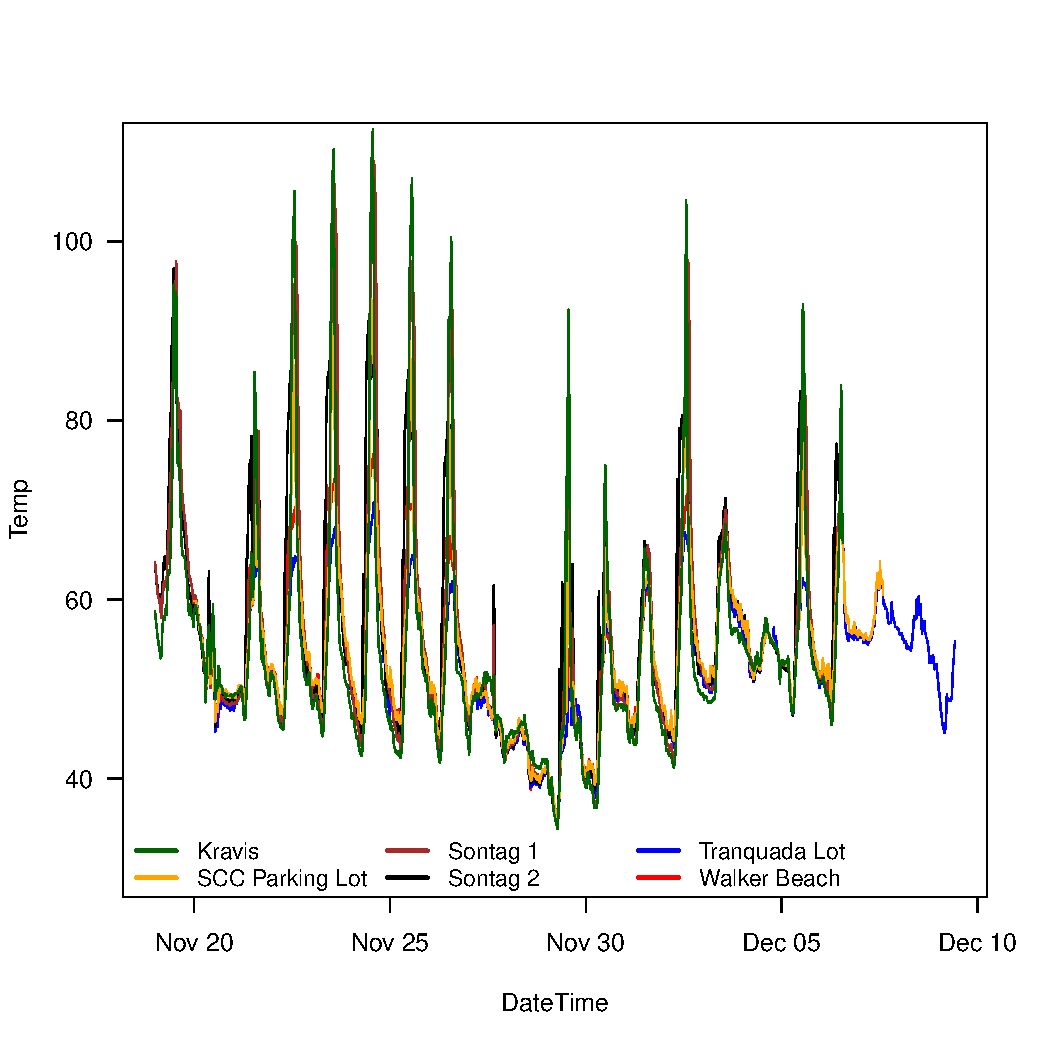
\includegraphics[width=\maxwidth]{figure/unnamed-chunk-5-1} 

\end{knitrout}
\caption{All time series in one graphic. Not easy to see what's going on.}
\label{fig.alldata}
\end{figure}

\subsection{Paired Plots -- Sun versus Shade}

First, we'll put everything in one graph (Figure~\ref{fig.paired}). Here we can see the spikes associated with the sunshine, which is not representative of ``weather'' records. 

\begin{figure}
\begin{knitrout}
\definecolor{shadecolor}{rgb}{0.969, 0.969, 0.969}\color{fgcolor}
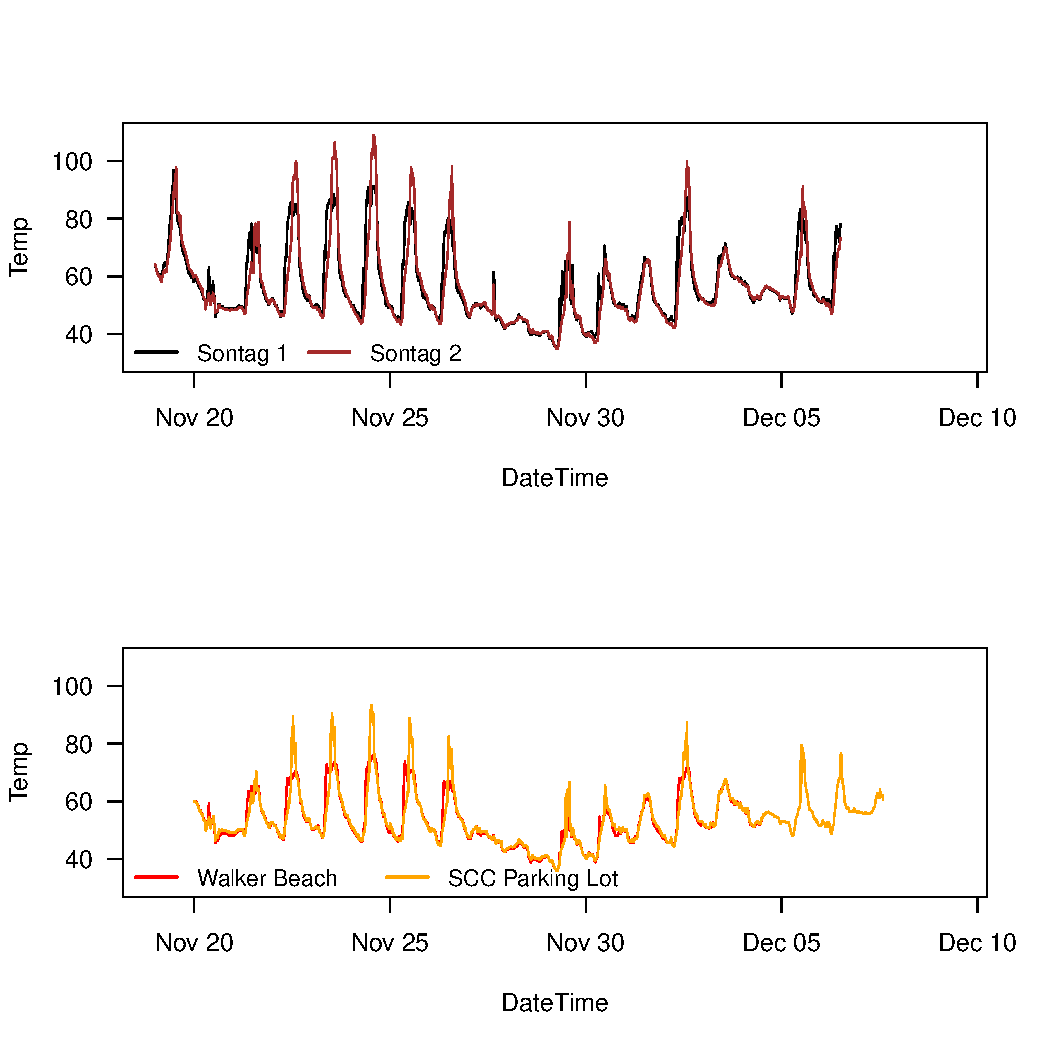
\includegraphics[width=\maxwidth]{figure/unnamed-chunk-6-1} 

\end{knitrout}
\caption{Just just two values seems to allow us with some capacity to distinquish the differences with more confidence.}
\label{fig.paired}
\end{figure}

\section{TMAX-TMIN and TAVE}

\begin{knitrout}
\definecolor{shadecolor}{rgb}{0.969, 0.969, 0.969}\color{fgcolor}\begin{kframe}
\begin{verbatim}
##         Date Location     TAVE    TMAX   TMIN
## 1 2019-11-19   Kravis 64.90554  95.207 53.449
## 2 2019-11-20   Kravis 52.93400  59.508 48.517
## 3 2019-11-21   Kravis 55.29337  85.374 46.548
## 4 2019-11-22   Kravis 58.33877 105.577 45.466
## 5 2019-11-23   Kravis 58.37640 110.264 44.742
## 6 2019-11-24   Kravis 57.38912 112.467 42.548
##         Date        Location     TAVE   TMAX   TMIN
## 1 2019-11-20 SCC Parking Lot 52.21220 59.851 46.369
## 2 2019-11-21 SCC Parking Lot 54.93791 70.480 48.160
## 3 2019-11-22 SCC Parking Lot 58.05701 89.384 47.088
## 4 2019-11-23 SCC Parking Lot 59.43398 90.680 47.446
## 5 2019-11-24 SCC Parking Lot 59.32753 93.493 46.188
## 6 2019-11-25 SCC Parking Lot 57.50675 88.833 46.188
\end{verbatim}
\end{kframe}
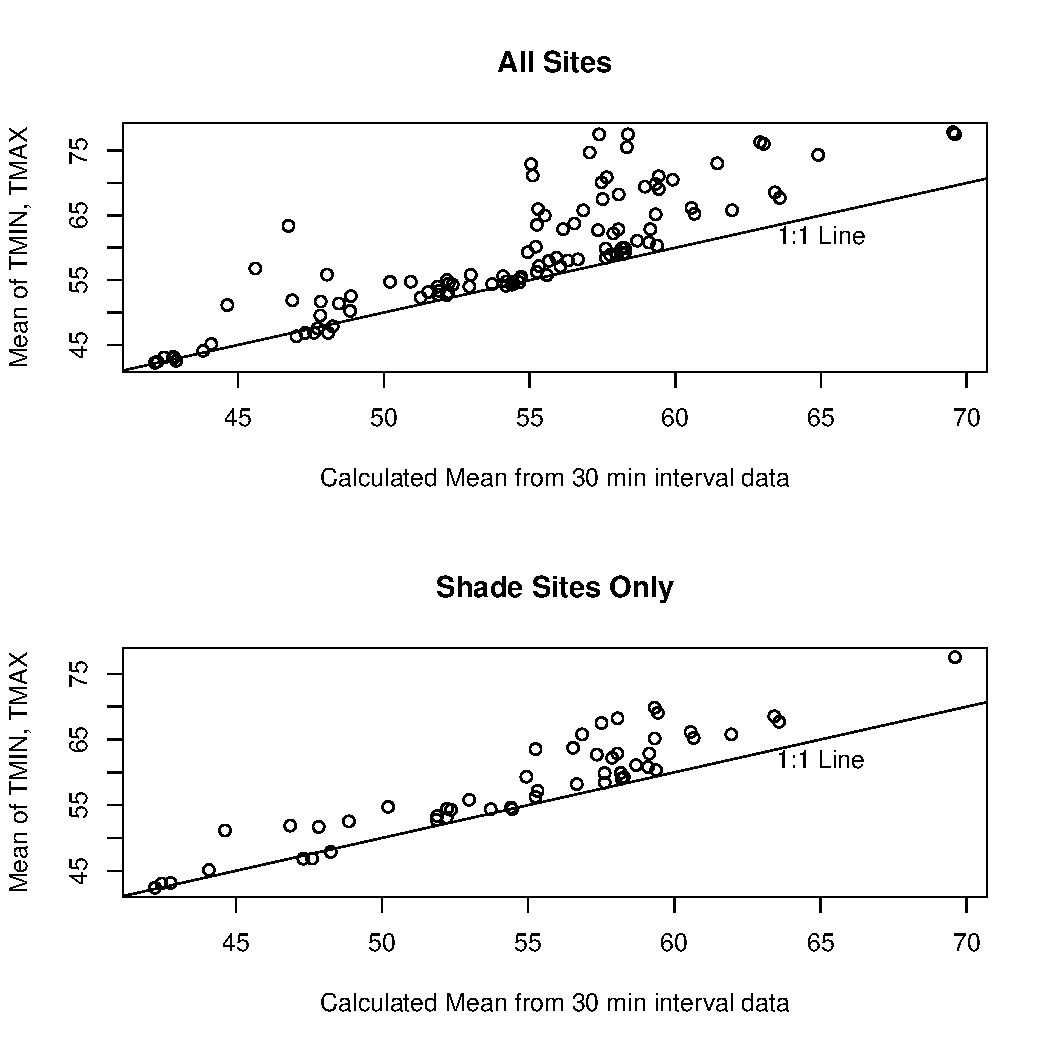
\includegraphics[width=\maxwidth]{figure/unnamed-chunk-7-1} 

\end{knitrout}





\end{document}
